\chapter{Numerische Lösung von Differentialgleichungen}
Bsp: Einschwinganalyse (TRansiente Analyse)

\begin{figure}
\center
\begin{circuitikz}
	\draw (2, 0) node[below] {0} to [R=$R$, i=\textcolor{red}{$i_R(t)$},*-*] (2, 4) node[above] {1};
	\draw (0, 0) to [I,i_=\textcolor{red}{$i_{0}(t)$}] (0, 4);
	\draw (4, 0) to [C=$C$, i=\textcolor{red}{$i_C(t)$}] (4, 4);
	\draw (0, 0) to [short] (4, 0);
	\draw (0, 4) to [short] (4, 4);
	\draw (4.5, 0) to [open,v=\textcolor{blue}{$y(t)$}] (4.5, 4);
\end{circuitikz} 

\caption{Beispielschaltung Transiente Analyse}
\end{figure}

\section{Analytische Lösung mittels Laplace-Transformation}
\begin{equation}
\begin{split}
C\cdot\dot{y}(t) + \frac{1}{R}\cdot y(t) &= i_0(t)\\
\dot{y}(t) + \underbrace{\frac{1}{RC}}_{-p_\infty}\cdot y(t) &= \frac{1}{RC}R\cdot i_0(t)\\
\dot{y}(t) - p_\infty y(t) &= -p_\infty R\cdot i_0(t)\\
\LT \text{Laplace}\\
p\cdot Y(p) - \underbrace{y(+0)}_{=0} - p_\infty Y(p) &= -p_\infty R\frac{1}{p}\cdot I_0\\
Y(p) &= \frac{-p_\infty R\cdot I_0}{(p-p_\infty)} = \frac{A}{p} + \frac{B}{p-p_\infty}
\end{split}
\end{equation}
\begin{equation}
A = \lim\limits_{p\rightarrow 0} p\cdot Y(p) = R\cdot I_0
\end{equation}
\begin{equation}
B = \lim\limits_{p\rightarrow p_\infty} (p-p_\infty)\cdot Y(p) = -R\cdot I_0
\end{equation}
\begin{equation}
\begin{split}
\LT\\
y(t) = A + B e^{p_\infty t} = R\cdot I_0\cdot (1-e^{p_\infty t})
\end{split}
\end{equation}

\section{Numerische Lösung mittels explizite Euler-Methode (linear Z-Transformation)}
\missingfigure{plot}
Diskretisierung der Zeit
\begin{equation}
y(\nu)\hat{=} y(\nu\cdot\Delta t) = y(t)
\end{equation}
Diskretisierung der DGL
\begin{equation}
\dot{y}(\nu)\approx p_\infty\cdot y(\nu) - p_\infty - p_\infty R\cdot i_0(\nu)
\end{equation}
Differenzengleichung (explizite Euler-Methode)
\begin{equation}
y(\nu+1)\approx y(\nu) + \Delta t\cdot\dot{y}(\nu)
\end{equation}

\missingfigure{plot}
\begin{equation}
y(\nu+1)\approx y(\nu) + \Delta t\cdot\left[p_\infty y(\nu) - p_\infty R\cdots i_0(\nu)\right]\quad ,\nu = 0,1,2,\ldots
\end{equation}
\begin{equation}
\hat{y}(\nu+1) = (1+p_\infty\Delta t)\cdot y(\nu) - \Delta t p_\infty R i_0(\nu)
\label{eq:y_dach}
\end{equation}
sukzessive Berechnung ausgehend von $y(0),\;\nu = 1,2,3,\ldots$

Bei linearen Schaltungen (linearen Differenzengleichungen) ist geschlossene numerische Lösung möglich durch $\ZT$ von \autoref{eq:y_dach}
\begin{equation}
z\cdot\dot{Y}(z)-\underbrace{z\cdot y(0)}_{0} - (1-p_\infty\Delta t)\cdot Y(z) = -p_\infty R\Delta t \frac{z}{z-1}I_0
\end{equation}
\begin{equation}
\begin{split}
Y(z) &= \frac{-p_\infty\Delta t R}{z-(1+p_\infty\Delta t)}\frac{zI_0}{z-1} = \frac{zRI_0}{z-1}\frac{zRI_0}{z-(1+p_\infty\Delta t)}\\
\ZT\\
\hat{y}(\nu) &= \left[1-(1+p_\infty\Delta t)^\nu\right]\cdot RI_0\quad ,\nu = 0,1,2,\ldots
\end{split}
\end{equation}

Zahlenbeispiel: $I_0R = 1;\;p_\infty = -1,\; t=1$\\
exakte Lösung: $y(1) = 1-e^{-1} = \num{0.632121}$\\
numerische Lösung: $y(\nu) = 1-(1-\Delta t^\nu\quad ,\nu\cdot\Delta t = 1$

\begin{tabular}{c|c|c|c}
$\Delta t$ & $\nu$ & $\dot{y}(1)$ & $\varepsilon^{(A)} = \abs{\hat{y}(1)-y(1)}$\\
\hline
\num{0.1} & \num{10} & \num{0.651322} & \num{0.019201}\\
\num{0.05} & \num{20} & \num{0.641514} & \num{0.009393}\\
\num{0.025} & \num{40} & \num{0.636768} & \num{0.004647}\\
\end{tabular}
$\quad$ Fehler $\varepsilon^{(A)}\sim \Delta t$

\textbf{Stabilität: }\\
\begin{tabular}{rrr}
Für & $|1+p_\infty \cdot \Delta t| = |1-\Delta t| < 1$ & $\Rightarrow \lim\limits_{x\rightarrow \infty} \hat{y}(\nu) = 1$\\
& $0 < \Delta t < 2$ & Algorithmus stabil\\
Für & $|1-\Delta t| > 1$ & $\Rightarrow \lim\limits_{v \rightarrow \infty} \hat{y}(\nu) \rightarrow \infty$ \\
& $\Delta t > 2$ & Algorithmus instabil
\end{tabular}

\section{Einfache numerische Integrationsverfahren}
\begin{equation}
\begin{split}
y(0) &= 0,\quad y(t) = \int\limits_0^t \dot{y}(\tau) \diff \tau\\
y(t+ \Delta t) &= \int\limits_0^t \dot{y}(\tau) \diff \tau + \int\limits_t^{t+\Delta t} \dot{y}(\tau) \diff\tau = y(t) + \int\limits_t^{t+\Delta t} \dot{y}(\tau) \diff\tau\\
y(\nu +1) &\approx y(\nu) + \tilde{\Delta y} = y(\nu) + \frac{\Delta t \cdot \tilde{\Delta y}}{\Delta t}
\end{split}
\end{equation}

\textbf{Expliziter Euler: } $y(\nu +1) \approx y(\nu) + \Delta t \cdot \dot{y}(\nu)$ (FE, Forward Euler)\\
\missingfigure{plot}\\

\textbf{Impliziter Euler: } $y(\nu +1) \approx y(\nu) + \Delta t \cdot \dot{y}(\nu +1)$ (BE, Backward Euler)\\
\missingfigure{plot}\\

\textbf{Trapez-Methode: } $y(\nu +1) \approx y(\nu) + \frac{\Delta t}{2} \cdot (\dot{y}(\nu) + \dot{y}(\nu + 1)$ (TR, Trapezvidal)\\
\missingfigure{plot}\\

\section{Eigenschaften numerischer Integrationsverfahren}
\begin{itemize}
\item explizit/implizit: wird Wert aus aktuellem Zeitschritt ($\nu + 1$) verwendet?
\item Schrittzahl: Anzahl der verwendeten vergangenen Zeitschritte
\item Genauigkeit: $\varepsilon^{(A)}(\nu \cdot \Delta t) = \hat{x}(\nu) - x(\nu) \approx (\Delta t)^k$\\
(für $|p_\infty \Delta t| << 1$) \quad Fehler der Ordnung $k$
\item Stabilität: \begin{itemize}
\item für $\Re{p_\infty} < 0$
\item für $\Delta t \rightarrow \infty$ ("'asymptotische Stabilität"')
\end{itemize}
\end{itemize}

\begin{tabular}{lll}
\textbf{Test-DGL:} & $\dot{x}(t) = p_\infty \cdot x(t)$ & $p_\infty$: Eigenwerte des Systems\\
& exakte Lösung: & $x(t) = x(0) \cdot e^{p_\infty t}$\\
&& $x(\nu) = x(0) \cdot e^{p_\infty \cdot \nu \cdot \Delta t},\ x(0) \neq 0$\\
& numerische Lösung: & $\hat{x}(\nu) = \int \{\hat{f}(\nu)\}$\\
& Fehler: & $\varepsilon^{(A)}(\Delta t) = \hat{x}(\nu) - x(\nu) = \hat{x}(\nu) - x(0) \cdot e^{p_\infty \nu \Delta t}$
\end{tabular}

\section{Expliziter Euler Eigenschaften}
\textbf{Differenzengleichung:} $\hat{x}(\nu +1) = \hat{x}(\nu) + \Delta t \cdot \hat{f}(\nu),\ f(t) = \dot{x}(t)$\\
Einschritt-Verfahren\\

\begin{tabular}{ll}
\textbf{Test-DGL:} & $f(t) = \dot{x}(t) = p_\infty \cdot x(t)$\\
& $x(0) \neq 0$\\
Differenzengleichung: & $\dot{x}(\nu +1) = \hat{x}(\nu) + \Delta t p_\infty \cdot \hat{x}(\nu) = (1 + p_\infty \cdot \Delta t) \cdot \dot{x}(\nu)$\\
numerische Lösung: & $\hat{x}(\nu) = (1+ p_\infty \Delta t) \cdot x(\nu)$\\
Genauigkeit: & $\varepsilon^{(A)} = \hat{x}(\nu) - x(\nu) = \Delta t \cdot \frac{\overbrace{\nu \Delta t}^{=t}}{2} \cdot p_\infty^2 \cdot x(0) \cdot e^{p_\infty \overbrace{\nu \Delta t}^{=t}}$ \\
Stabilität: & $\lim_{t \rightarrow \infty} x(t) \rightarrow 0$ für $\Re{p_\infty} < 0$ \\
& $\lim_{\nu \rightarrow \infty} \hat{x}(\nu) = \lim_{\nu \rightarrow \infty} (1 + p_\infty \Delta t)^\nu x(0) \rightarrow 0$ falls $|1 + p_\infty \Delta t| < 1|$ \\
Ordnung & $k=1$ \\
Asymptotische Stabilität ($\Delta t \rightarrow \infty$): & $\hat{x}(\nu + 1) \approx p_\infty \Delta t \hat{x}(\nu) \Rightarrow$ instabiles Verhalten!
\end{tabular}

\begin{figure}
\center
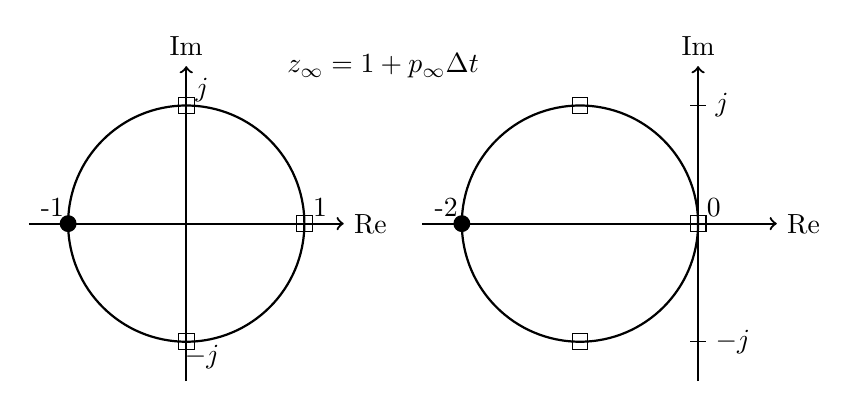
\begin{tikzpicture}
	\node at (2.5,2) {$z_\infty = 1 + p_\infty\Delta t$};

	\draw[thick,->] (-2,0) -- (2,0) node[right]{Re};
	\draw[thick,->] (0,-2) -- (0,2) node[above]{Im};
	\draw[thick] (0,0) circle (1.5);
	\draw (1.4,-0.1) rectangle (1.6,0.1) ++ (.1,.1) node {1};
	\draw (-0.1,1.4) rectangle (0.1,1.6) ++ (.1,.1) node {$j$};
	\filldraw (-1.5,0) circle (0.1) ++ (-.2,.2) node {-1};
	\draw (-0.1,-1.4) rectangle (0.1,-1.6) ++ (.1,-.1) node {$-j$};
	
	\draw[thick,->] (3,0) -- (7.5,0) node[right]{Re};
	\draw[thick,->] (6.5,-2) -- (6.5,2) node[above]{Im};
	\draw[thick] (5,0) circle (1.5);
	\draw (6.4,1.5) -- (6.6,1.5) node[right] {$j$};
	\draw (6.4,-1.5) -- (6.6,-1.5) node[right] {$-j$};
	\draw (6.4,-0.1) rectangle (6.6,0.1) ++ (.1,.1) node {0};
	\draw (4.9,1.4) rectangle (5.1,1.6);
	\filldraw (3.5,0) circle (0.1) ++ (-.2,.2) node {-2};
	\draw (4.9,-1.4) rectangle (5.1,-1.6);
	
\end{tikzpicture} 

\caption{Stabilitätsbereich für den expliziten Euler}
\end{figure}

Somit ist die Wahl von $\Delta t$ aus Stabilitätsgründen eingeschränkt. Bei zu großem $\Delta t$ liegt das Produkt $p_\infty \Delta t$ nicht mehr im Stabilitätsbereicht. Praktisch beim expliziten Euler ist hingegen, dass es keine Stabilität in der rechten Halbebene gibt, es werden also instabile System als instabil detektiert.

Im folgenden noch einmal die Eigenschaften der Verfahren kurz zusammengefasst:

\begin{tabular}{r|c|c|c|p{2.2cm}|p{2.3cm}}
& explizit/implizit & Schritte & Ordnung & stabil für $\Re{p_\infty} < 0$ & asymptotisch stabil \\ \hline
expliziter Euler & explizit & 1 & 1 & nein & nein \\ \hline
impliziter Euler & implizit & 1 & 1 & ja & ja \\ \hline
Trapez & implizit & 1 & 2 & ja & nein \\ \hline
Gear & implizit & 2 & 2 & ja & ja
\end{tabular} \hfill \\
Zudem haben Einschrittverfahren Vorteile beim Starten, mit Mehrschrittverfahren kann nicht direkt gestartet werden.

\section{Taylor-Verfahren höherer Ordnung}
Die eher im technischen Bereich gängige Schreibweise
\begin{equation}
y(\nu + 1) = y(\nu) + \Delta t T^{(n)}(\nu, y(\nu))
\end{equation}
ist äquivalent zur in der Mathematik üblichen Variante
\begin{equation}
y_{i + 1} = y_i + h T^{(n)} (t_i, y_i)
\end{equation}
mit
\begin{equation}
T^{(n)}(t_i, y_i) = f(t_i, y_i) + \frac{h}{2} f'(t_i, y_i) + \dots + \frac{h^{n - 1}}{n!} f^{(n - 1)}(t_i, y_i)
\end{equation}

Dadurch erhält man einer bessere Genauigkeit, genauer gesagt: $\epsilon O(h^n)$. Nachteilig kann sich allerdings auswirken, dass höhere Ableitungen der Funktion benötigt werden.

\section{Prädiktor-Korrektor-Ansätze}
Die Grundidee dahinter ist ein explizites Verfahren zur Vorhersage des Wertes $y_{i + 1}$ zu nutzen, und diesen Werte nachträglich mithilfe eines weiteren Verfahrens zu verbessern. Dieser Ansatz kann auch iterativ verwendet werden.

Ein Beispiel für so einen Prädiktor-Korrektor-Ansatz ist das Verfahren von Heun, welches auf einem expliziten Euler basiert. Der explizite Euler liefert
\begin{equation}
y_{i + 1}^0 = y_i + h \cdot f(t_i, y_i)
\end{equation}
und daraus berechnet Hoin ein verbessertes
\begin{equation}
y_{i + 1}^1 = f(t_{i + 1}, y_{i + 1}^0) .
\end{equation}

Der iterativer Ansatz dazu wäre dann
\begin{equation}
y_{i + 1}^0 = y_i + h \cdot f(t_i, y_i)
\end{equation}
\begin{equation}
y_{i + 1}^j = y_i^m + h \cdot \frac{f(t, y_i^m) + f(t_{i + 1}, y_{i + 1}^{j - 1}}{2}
\end{equation}

\section{Adams-Bashforth/Adams-Moulton}
Die Grundidee hinter diesen Verfahren beruht darauf $f$ durch ein Interpolationspolynom zu ersetzen.

Ausgangspunkt ist die Differentialgleichung
\begin{equation}
y' = f(t, y)
\end{equation}
wobei $a \le t \le b$ und $y(a) = \alpha$.

Adams-Bashforth und Adams-Moulton sind $m$-schrittige Mehrschrittverfahren, in denen $y_{i + 1}$ ersetzt wird durch 
\begin{equation}
y_{i + 1} = a_{m - 1} y_i + a_{m - 2} y_{i - 1} + \dots + a_0 y_{i + 1 - m} + h \left[ b_m f(t_{i + 1}, y_{i + 1}) + b_{m - 1} f(t_i, y_i) + \dots + b_0 f(t_{i + 1 - m}, y_{i + 1 - m}) \right]
\end{equation}
mit $i = m - 1, m, \dots N - 1$, $h = \frac{b - a}{N}$. Falls $b_n = 0$ spricht man von einem expliziten Verfahren, ansonsten von einem impliziten.

\paragraph{Herleitung}
\begin{equation}
y(t_{i + 1}) = y_{i + 1}
\end{equation}
\begin{equation}
y_{i - 1} - y_i = \int_{t_i}^{t_{i + 1}} y'(t) \diff t = \int_{t_i}^{t_{i + 1}} f(t_i, y(t)) \diff t
\end{equation}
\begin{equation}
y_{i + 1} = y_i + \int_{t_i}^{t_{i + 1}} f(t_i, y(t)) \diff t
\end{equation}
Ersetze $f(t_i, y(t)) $ durch Interpolationspolynom $P(t)$
\begin{equation}
y_{i + 1} \approx y_i + \int_{t_i}^{t_{i + 1}} P(t) \diff t
\end{equation}

Für das Interpolationspolynom bieten sich an
\begin{itemize}
\item Taylor
\item Lagrange
\item Newton'sche Rückwärtsdifferenzen
\end{itemize}

\subsection{Adams-Bashforth (explizit)}
Die explizite Einschrittvariante ist äquivalent zum expliziten Euler:
\begin{equation}
y_{i + 1} = y_i + h f(t_i, y_i)
\end{equation}
Die Variante mit zwei Schritten lautet
\begin{equation}
y_{i + 1} = y_i + \frac{h}{2} \left[ 3 f(t_i, y_i) - f(t_{i - 1}, y_{i - 1} \right]
\end{equation}
und hat eine quadratisches Fehlerverhalten.

\subsection{Adams-Moulton (implizit)}
Die Einschrittvariante hiervon ist für $m = 0$ der implizite Euler, für $m = 1$ das Trapezverfahren. Wenn zwei Schritten verwendet werden sieht das Verfahren wie folgt aus
\begin{equation}
y_{i + 1} = y_i + \frac{h}{12} \left[ 5 f(t_{i + 1}, y_{i + 1} + 8 f(t_i, y_i) - f(t_{i - 1}, y_{i - 1}) \right]
\end{equation}
und besitzt ein kubisches Fehlerverhalten. 
